Mobile Geräte sind heutzutage ein sehr großer Teil unseres Tagesablaufs. Durchschnittlich verbringen wir 3:54 Stunden pro Tag an mobilen Geräten (hier bezogen aus Bürger der USA). Die meiste Zeit hiervon wird in Apps (ca. 90\%). \footnote{\url{https://www.emarketer.com/content/us-time-spent-with-mobile-2019}, zuletzt aufgerufen: 26.02.2021} 
Laut Cisco wird dieser Markt sich jedoch nicht nur auf Industrieländer beruhen, sondern bis 2023 sollen weltweit 71\% der Bevölkerung mobile Konnektivität haben. \cite{cisco2020}
Diese Entwicklung forcierte viele Firmen immer mehr ihre Anwendungen auch \textit{mobile ready} zu gestalten. Dies kann man bspw. deutlich bei der Anpassung vieler Webseiten an Mobile Seiten- und Größenverhältnisse oder auch dem Anbieten von \textit{Apps}, welche bereits für Desktop o.ä. verfügbar waren, erkennen. \\

Daher ist es für die Wirtschaft und Entwicklung gleichermaßen wichtig sich ständig weiterzuentwickeln und sich nicht auf (Kosten-) ineffiziente Entwicklungsprozesse auszuruhen. Dabei bieten jährliche, wenn nicht sogar halbjährliche Design- und Performanceänderungen von den Geräten selbst oder der Betriebssysteme Herausforderungen an die mobilen Anwendungen - \textit{apps} - und gleichzeitig an deren Programmierumgebung. Trotz einer riesigen Auswahl an \textit{Apps} lassen sich diese allgemein in drei Kategorien eingliedern: Plattformspezifische native Anwendungen, adaptive Webanwendungen und plattformübergreifende Anwendungen.

\subsubsection{Begriffe}
\subparagraph{Eine Plattform} besteht aus der Hardware (System und zusätzlicher Peripherie, wie Sensoren oder Aktoren), dem Betriebssystem, den spezifischen \textit{Software Development Kits (SDK)} und den jeweiligen Basisbibliotheken. 
Zusammen bietet eine Plattform die Grundlage um Software für sie zu entwickeln.
\subparagraph{Ein \textit{Framework}} definiert eine Architektur für Anwendungen und stellt Komponenten bereit, mit welchen das Entwickeln einer Anwendung erleichtert sein soll. \cite{johnson1988} 
Ein plattformübergreifendes Framework muss somit Anwendungscode für mehrere Plattformen wiederverwenden, jedoch müssen auch plattformspezifische Funktionen, wie Architektur oder Benutzeroberflächen API, bereitgestellt werden. Mehr dazu in Kapitel \ref{plattformuebergreifende_anwendungen}.

\subparagraph{Eine mobile Anwendung} ist eine Anwendung, geschrieben für eine Plattform eines mobilen Endgerätes, welche die jeweiligen Features nutzen könnte - dazu zählen Kamera(s), Beschleunigungssensoren oder auch \textit{Global Positioning System (GPS)}. Webseiten als solches sind demnach keine mobilen Anwendungen.


\subsubsection{Plattformspezifische native Apps}
Plattformspezifische oder auch native Anwendungen sind Programme, welche auf eine gewisse Plattform abzielen und in einer der davon unterstützen Programmiersprachen geschrieben wurden. Da diese Art der (mobilen) Anwendung mit plattformspezifischen  SDK und \textit{Frameworks} entwickelt wird, ist diese Anwendung an eine Plattform gebunden. \\
Dies bringt zum einen natürlich Vorteile wie allgemein best mögliche Performance auf der jeweiligen Plattform und direkt vom Hersteller unterstützte Entwicklungsumgebungen/SDKs.
Zudem lassen sich plattformspezifische Fähigkeiten oder Einstellungen nutzen - beispielsweise mehrere Kameras oder GPS.

Gleichzeitig beschränkt man sich aber logischerweise auf eine Plattform und deckt mit einer Anwendung nur einen Teil des gesamten Marktes. Dies bringt im Vergleich zu den anderen Möglichkeiten einen deutlich erhöhten Entwicklungs- und Wartungsaufwand mit sich, da für andere Plattformen Programmcode nicht übernommen werden kann. Zusätzlich benötigen Entwickler spezifische Kompetenzen für beide Plattform und Entwicklungsumgebungen. \\

Zwei der am weitesten verbreiteten Plattformen sind Android von Google und iOS von Apple. Anwendungen für Android können in Kotlin oder Java als Programmiersprache beispielsweise in dem \textit{integrated development environment (IDE)} von Google Android Studio entwickelt werden. Für iOS wird hingegen mit Objective-C und Swift als Programmiersprache primär in der IDE XCode entwickelt.

Beide bieten jeweils Plattform eigene Services an, beispielsweise das direkte Veröffentlichen in den jeweiligen Appstore \cite{fentaw2020}

\subsubsection{Plattformübergreifende Anwendungen}
\label{plattformuebergreifende_anwendungen}
Die Entwicklung einer plattformübergreifenden Anwendung zeichnet sich generell durch die Möglichkeit aus, nur einmal Code schreiben zu müssen, diesen jedoch auf mehreren Plattformen ausführen zu können. \\
Verschiedene Ansätze einer solchen Anwendung sind in Abbildung \ref{fig:crossplattform_architecture} kategorisiert. Im Folgenden werden jene Entwicklungsmöglichkeiten detaillierter besprochen.

\begin{figure}[h]
	\begin{center}
		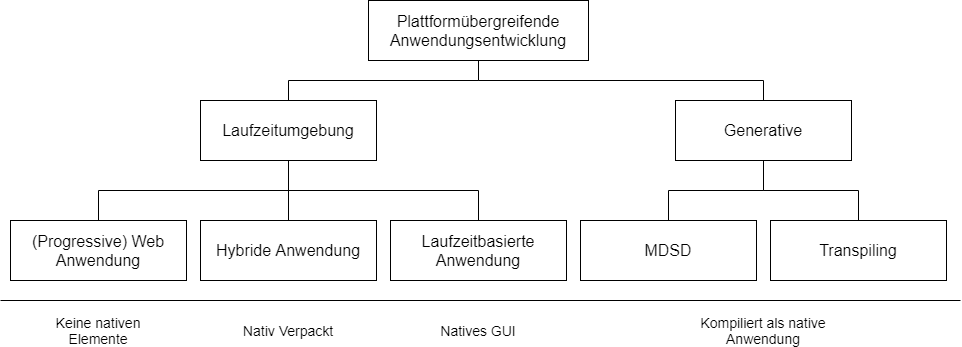
\includegraphics[scale=0.47]{Theoretische_Grundlagen/images/crossplattform_unterteilung.png}
	\end{center}
	\caption{Kategorisierung verschiedener plattformübergreifender Ansätze. Erstellt nach \cite{majchrzak2015} \protect}
	\label{fig:crossplattform_architecture}
\end{figure}

\paragraph{\textit{(Progressive) Web Apps}}
Eine mobile Webanwendung ist eigentlich eine Webseite, welche sich an die Größe und Auflösung von unterschiedlichen Bildschirmen anpasst - hier speziell an die Bildschirmgrößen der mobilen Geräte. Diese Anwendung ist mit Standard Webentwicklungstools geschrieben (HTML, CSS \& JavaScript) und läuft somit theoretisch auf jedem Gerät mit einem Internet Browser. \cite{charland2011}
Aufgrund der steigenden Unterstützung von jeglichen APIs in mobilen Browsern, ist es auch möglich geworden auf Geräteeigenschaften, wie bspw. den Standort zuzugreifen.\\
Jedoch kann diese App logischerweise nicht im jeweiligen \textit{Appstore} heruntergeladen werden, da es sich weiterhin um eine Webseite handelt.
Aus gleichem Grund kann hiermit auch kein \glqq natives Design und Leistung\grqq erzeugt werden.\\

Abhilfe hierfür sorgt jedoch die von Google vorgestellte Design Idee \textit{Progressive Web Apps} (PWA). Sie bietet die Möglichkeit Code in sog. \textit{service worker} als Hintergrundthread ausführen zu lassen, ein Webseiten Manifest anzugeben, die App offline bedienen zu können und bieten die Möglichkeit die PWA zu installieren. Gleichzeitig kann mit diesem Design eine zu nativen Apps vergleichbare Leistung erreicht werden.\cite{bjorn-hansen2020} \\

Generell ist der Ansatz sehr simpel, da hiermit plattformübergreifende Anwendungen geschrieben werden können, welche sich auf allen Geräten mit Browser bedienen lassen. 
Hierfür wird zudem keine zusätzliche Programmiersprache oder wissen über die jeweilige Plattform benötigt.\\
Eine große Schwierigkeit hieran ist weiterhin der Zugriff auf Gerätefeatures, da nicht alle über den Browser verfügbar sind.

\paragraph{Hybride Anwendungen}
\label{hybride_anwendung}
Eine hybride Anwendung kombiniert die native Vorgehensweise mit der einer normalen Webseite. 
In einer nativen WebView ist eine Webanwendung verpackt, welche nun in einer \textit{HTML-Rendering-Engine} gerendert wird. Bei Android und iOS ist das WebKit.
Diese WebView funktioniert ähnlich wie ein normaler Browser, jedoch werden Kontrollfenster nicht angezeigt, wie zum Beispiel Adresszeile, Einstellungen oder Lesezeichen.
Ähnlich wie bei Web Anwendungen werden über JavaScript APIs Gerätefeatures eingebunden.\\
Ein sehr frühes Framework für diese Art von Anwendung war \href{https://cordova.apache.org/}{Adobe Cordova}, eher bekannt als das ursprüngliche PhoneGap von Nitobi. Viele weitere Frameworks basieren auf ihren Anfängen.\\

Eine hybride Anwendung kann also normal als App im \textit{Appstore} heruntergeladen auf dem Gerät installiert und offline genutzt werden - also sehr ähnlich zu nativen Lösungen. Daher ist dieser Ansatz auch sehr beliebt 
Daher liegt auch hier die Leitung der Applikation deutlich hinter der der Nativen. \cite{lachgar2017} \cite{bjorn-hansen2020}

\begin{figure}[tbt]
	\begin{center}
		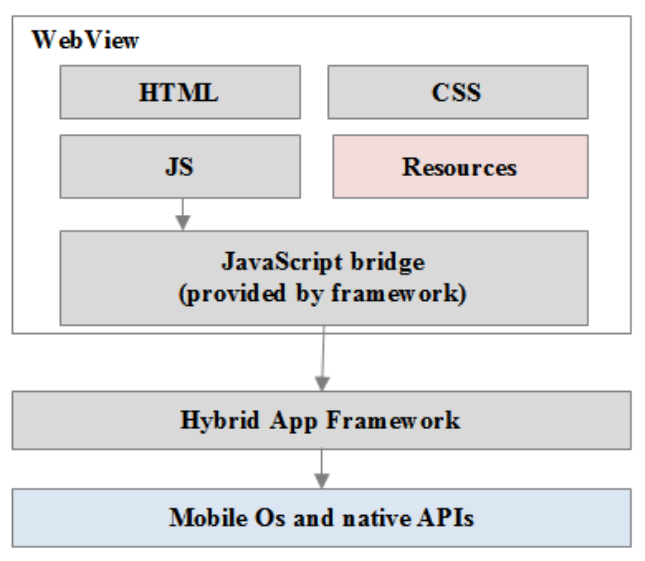
\includegraphics[scale=0.45]{images/hybride-anwendungen-struktur.PNG}
	\end{center}
	\caption{Struktur einer hybriden Anwendung \protect \footnotemark}
	\label{fig:hybrid_structure}
\end{figure}
\footnotetext{Quelle: \cite{lachgar2017}}

\paragraph{Runtime basierte Anwendungen}
\label{runtime_based_apps}
Im Gegensatz zur in Kapitel \ref{hybride_anwendung} beschriebenen hybriden Anwendung, nutzen Runtime basierte Anwendungen keinen Browser des Gerätes mit einer WebView, sondern jede App besitzt eine eigene Runtime Ebene. 
Jedes Framework muss also eine solche Ebene für alle Plattformen in jeweiliger Programmiersprache mitliefern, damit seine Anwendung hierauf laufen können.
Die Anwendungen hingegen sind dann beispielsweise in JavaScript (bspw. \href{https://reactnative.dev/}{React Native} oder \href{https://nativescript.org/}{NativeScript}), C\# (\href{https://dotnet.microsoft.com/apps/xamarin}{Xamarin}) oder sonstigen Programmiersprachen (bspw. \href{https://www.qt.io/}{Qt}) geschrieben.\\
\\
Jedem Framework-Entwickler ist die Freiheit gegeben, wie man die Anbindung an native Funktionen regelt. Bei hybriden Anwendungen ist dies durch die WebView Cordova festgelegt.
Typisch für Anwendungen dieser Art jedoch ist ein Plug-In-basiertes \textit{bridging System}. Es ermöglicht den Aufruf von fremden Funktionsinterfaces in plattformspezifischem Code.
Somit können beispielsweise React Native und NativeScript mit Sprachinterpretern (bspw. JavaScriptCore und V8) auf den Geräten Auszeichnungssprache (hier HTML (Hypertext Markup Language)) interpretieren und plattformspezifische Komponenten der Benutzeroberflächen erzeugen.\\
\\
Ein großer Nachteil dieser Strategie ist jedoch zugleich ihr Vorteil: Jedes Framework besitzt seine eigene Architektur. Dadurch sind Plug-ins des einen Frameworks trotz gleicher Anwendungssprache nicht unbedingt funktionstüchtig im anderen. 
Bei projektspezifischen Plug-ins macht es einen späteren Systemwechsel daher besonders schwer, da nicht nur Benutzeroberfläche und Businesslogik neu geschrieben werden müssen, sondern auch jeweilige Plug-ins. \cite{bjorn-hansen2020}

\paragraph{Model-driven Software Entwicklung}
Die Grundsätze der modellgetriebenen Softwareentwicklung beschäftigen sich mit der Abstraktion des Modells als (Teil eines) System, von welchem die eigentliche Software abgeleitet wird. \cite{stahl2006}\\
Das bedeutet in der Realität, dass eine höhere Abstraktion als Quellcode in Form von textuellen oder grafischen domänenspezifischen Sprachen oder universell einsetzbaren Modellierungssprachen (Unified Modeling Language(UML)) zum beschreiben der Software verwendet wird. 
Codegeneratoren übersetzen diese Modelle nun jeweils in Programmiersprachen der gewählten Zielplattform, auf welcher sie kompiliert werden.\\
\\
Theoretisch kann dadurch der komplette Funktionsumfang wie bei einer nativen Anwendung erreicht werden.
Bekannte Frameworks dieser Methode sind zum Beispiel \href{https://www.wi.uni-muenster.de/sites/wi/files/public/department/pi/publications/heitkoetter/cross-platform-model-driven-development-of-mobile-applications-with-md2.pdf}{$M\!D_2$},\href{https://www.sciencedirect.com/science/article/abs/pii/S1477842417301215}{MAML}, \href{https://www.webratio.com/site/content/en/home}{WebRatio Mobile}, \href{https://www.biznessapps.com/}{BiznessApps} und \href{https://bubble.io/}{Bubble}.\\
\\
Der große Nachteil hieran ist, dass Entwickler sehr selten modellgetriebene Entwicklung verwenden, sondern Quellcode-basierte Programmiermethoden bevorzugen. \cite{bjorn-hansen2020}
\paragraph{Kompilierte Anwendungen}
\label{compilierte_anwendungen}
Kompilierte plattformübergreifende Anwendungen basieren auf einer einzigen Codebasis und können für mehrere Plattformen vollständig kompiliert werden. 
Dies kann entweder von der Codebasis einer nativen Anwendung für mindestens eine andere Plattform (bspw. \href{https://developers.google.com/j2objc/}{J2ObjC}), oder von einer unabhängigen Codebasis direkt für mehrere Plattformen (bspw. \href{https://flutter.dev/}{Flutter}) geschehen.
Hierbei ist Flutter für diesen Anwendungsfall am interessantesten und wird in Kapitel \ref{flutter} näher behandelt.\\
Ein Hindernis dieser Art ist die erhöhte Komplexität der einzelnen Frameworks.

\subsection{Frameworks zur mobilen, plattformübergreifenden Entwicklung}
In den folgenden Kapiteln werden einzelne Frameworks zur mobilen, plattformübergreifenden Entwicklung vorgestellt.\\
In der Statistik \ref{fig:crossplattform_popularity} aus dem Jahr 2020 ist React-Native das beliebteste Framework, dicht gefolgt von Flutter. 
Wie man deutlich hier auch sehen kann, haben andere, bisher auch sehr erfolgreiche Frameworks einen enormen Rückgang von teilweise über einem Drittel ihrer Nutzer erleben müssen. \\
\\
Aus diesen Gründen werden im weiteren Verlauf nur die Frameworks React-Native und Flutter weiter besprochen.

\begin{figure}[H]
	\begin{center}
		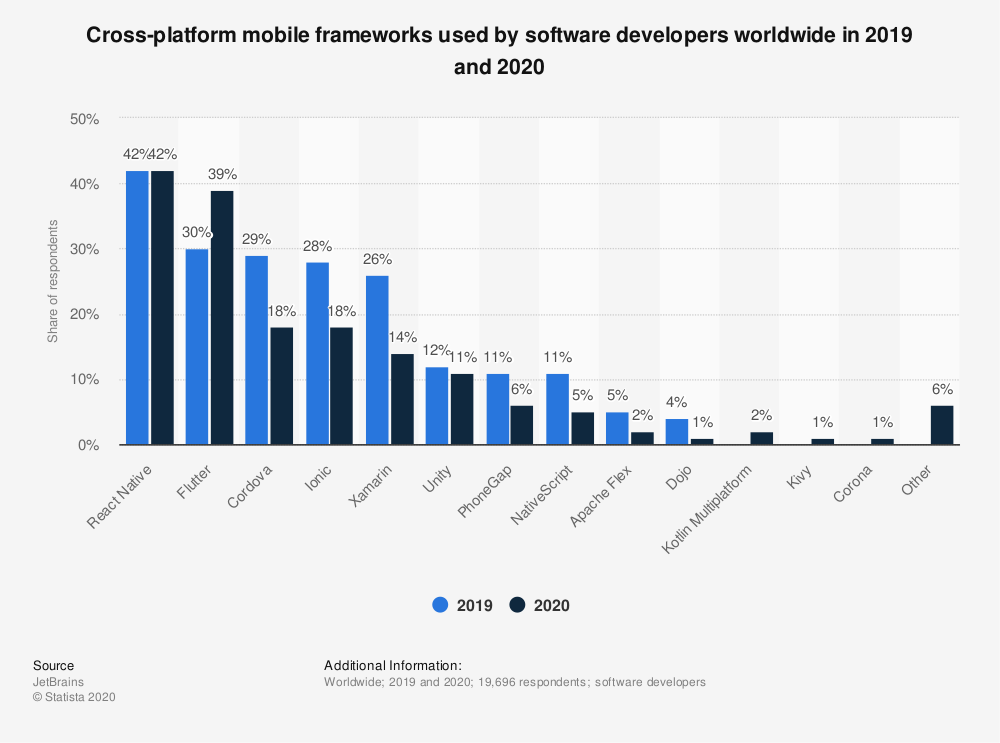
\includegraphics[scale=0.4]{Theoretische_Grundlagen/images/crossplattform_popularity.png}
	\end{center}
	\caption{Beliebtheit nach Framework im Bereich der plattformübergreifenden mobilen Entwicklung \protect \footnotemark}
	\label{fig:crossplattform_popularity}
\end{figure}
\footnotetext{Quelle: \href{https://www.statista.com/statistics/869224/worldwide-software-developer-working-hours/}{www.statista.com}, zuletzt aufgerufen am 22.04.2021}

\subsubsection{React Native}
\label{react-native}
React Native ist ein open source Framework, welches von Facebook 2015 veröffentlicht wurde. 
Es basiert auf dem bekannten Web-Framework \href{https://reactjs.org/}{\textit{React}} (ebenfalls von Facebook) und bringt daher den deklarativen und Komponenten-basierten Stil mit sich. 
Die Programmiersprache ist aus diesem Hintergrund auch logischerweise JavaScript.
Das Framework an sich ist in verschiedenen Sprachen implementiert: JavaScript, Swift, Objective-C, C++ und Python.\\
\\
Allgemein bietet das Framework die Möglichkeit plattformübergreifende Apps für iOS, Android und für Windows zu schreiben. Hierbei wird der geschriebene Code in einer JavaScript Laufzeitumgebung ausgeführt (React Native selbst verwendet generell \href{https://trac.webkit.org/wiki/JavaScriptCore}{JSC (JavaScriptCore)}, seit neuestem kommt auch \href{https://hermesengine.dev/}{Hermes} zum Einsatz, jedoch sind auch andere bekannte Umgebungen denkbar - bspw. \href{https://v8.dev/}{V8} in Chrome) es lässt sich zu den Runtime-basierten Anwendungen in Kapitel \ref{runtime_based_apps} zuordnen. \cite{reactnative2021}\\
\paragraph{Architektur}
Grundlegend wurde React Native als Plattform-agnostisch designet. Entwickler schreiben also plattformunabhängigen JavaScript React Code, während das Framework den erstellten React Baum in Plattform-spezifischen Code umschreibt. Hierbei wurde 2013 (noch intern) die Web-Technologie React mit nativen Plattformen (nur interne) vereint, jedoch war dieses Design aufgrund eines einzigen Threads sehr langsam. Um dies zu verbessern basierte das Framework lange Zeit auf drei unterschiedlichen Threads, welche über eine Brücke verbunden sind.

\begin{figure}[h]
	\begin{center}
		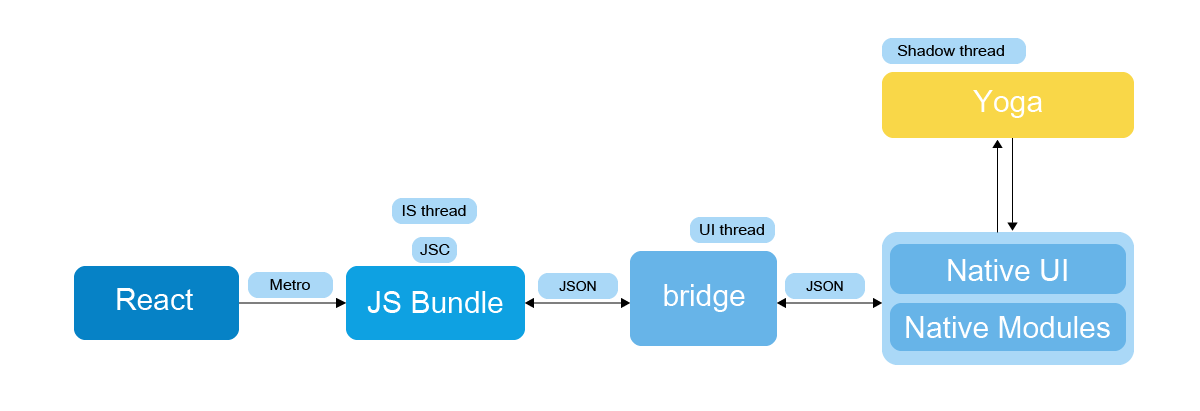
\includegraphics[scale=0.4]{Theoretische_Grundlagen/images/reactnative_architecture_old.png}
	\end{center}
	\caption{Alte Architektur von React Native \protect \footnotemark}
	\label{fig:reactnative_architecture_old}
\end{figure}
\footnotetext{Quelle: \href{https://litslink.com/blog/new-react-native-architecture}{React Native Re-Architecture}, zuletzt aufgerufen am 15.04.2021}

\begin{itemize}
	\item \textit{JavaScript Thread}. Hier wird der gesamte JavaScript Code abgelegt und interpretiert. Alles wird über die JSC Engine ausgeführt.
	\item \textit{Native Thread}. Die Benutzeroberfläche und Kommunikation mit dem JavaScript Thread steht hier im Mittelpunkt. Der gesamte native Code wird hier ausgeführt. Die Benutzeroberfläche wird dann aktualisiert, sobald die eben ein Änderung vom JS Thread vermittelt wird.
	\item \textit{Shadow Thread}. Hier wird das gesamte Layout der Anwendung berechnet. Zugrunde liegt die Facebook-eigene layout engine \glqq Yoga\grqq .
\end{itemize}

Ein Hauptproblem dieses Ansatzes ist, dass die Brücke grundlegend eine asynchrone Warteschlange ist, da der JS Thread und der native Thread unabhängig voneinander arbeiten. Zusätzlich werden während der gesamten Datenübertragung die Daten im JSON Format serialisiert und deserialisiert .
Daher kann es zu Performance-Einbrüchen und somit zu schlechter Nutzererfahrung, durch bspw. Eingabeverzögerung, kommen.

\begin{figure}[h]
	\begin{center}
		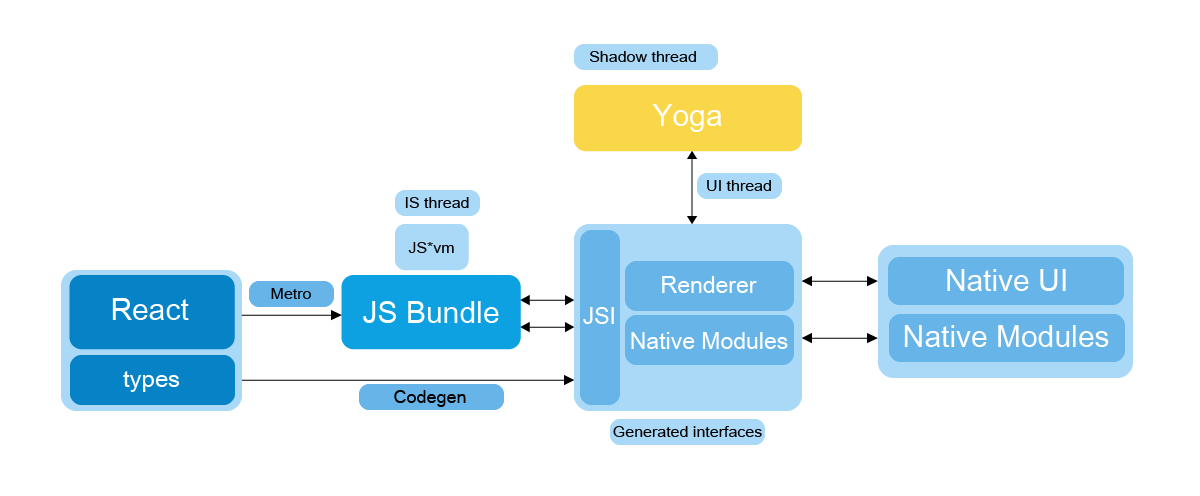
\includegraphics[scale=0.4]{Theoretische_Grundlagen/images/reactnative_architecture.png}
	\end{center}
	\caption{Neue Architektur von React Native \protect \footnotemark}
	\label{fig:reactnative_architecture}
\end{figure}
\footnotetext{Quelle: \href{https://litslink.com/blog/new-react-native-architecture}{React Native Re-Architecture}, zuletzt aufgerufen am 15.04.2021}

Nach der Ankündigung 2018 veröffentlichte Facebook im Juli 2020 die neue Architektur. Mit ihr wurde der Bottleneck (die Brücke) ersetzt durch das JavaScript Interface. 
Es ermöglicht nicht nur die komplette Synchronisierung der beiden Threads, sondern auch die direkte Kommunikation untereinander - vor allem das Konzept von \glqq shared ownership\grqq ist hier tragend, weshalb auch keine Serialisierung mehr nötig ist.
Zudem  ist man nun nicht mehr an JSC gebunden, sondern kann auch jegliche hoch-performante JavaScript Engines als Laufzeitumgebung verwenden.
Native Module werden nun nur noch bei Bedarf geladen anstatt alle beim Start der App.\\
Weiter wurde veralteten Legacy-Code aus dem Kern von React Native entfernt und nicht-essenzielle Teile aus dem Kern ausgelagert. Dadurch zeigt sich die aktuelle Architektur von React Native in Abbildung \ref{fig:reactnative_architecture}.\footnote{Quelle: \href{https://medium.com/swlh/react-natives-re-architecture-in-2020-9bb82659792c}{React Native's re-architecture in 2020}}

\paragraph{JSX mit nativen Komponenten}
React (Native) verwendet als Programmiersprache JSX. Diese ist eine syntaktische Erweiterung von JavaScript (\textbf{J}ava\textbf{S}cript e\textbf{X}tention), welche zur fundamentalen Beschreibung der Nutzeroberfläche dient. JSX wird in normale JavaScript Objekte kompiliert, weshalb es nicht zwingend ist. \\
\begin{lstlisting}[caption=JSX Hello World Element]
	const element = <h1>Hello, world!</h1>;
\end{lstlisting}
Mithilfe dieser losen Kopplung von UI-Code und dazugehöriger Logik schlägt React eine optionale Lösung zur \textit{Separation of Concerns} vor. Anstelle dessen ist es auch möglich die Technologien in Markup- und Logik-Dateien aufzuteilen. \\
Außerdem könnte man argumentieren, das JSX einfach eine weitere Template-Sprache sei - ähnlich HTML oder XAML. Jedoch ist dies falsch, da (wie oben bereits erwähnt) JSX lediglich eine syntaktische Erweiterung von JavaScript ist, also man inmitten von JSX Objekten JavaScript schreiben kann.\\
Weiterhin ist interessant, dass JSX \href{https://owasp.org/www-community/attacks/xss/}{Cross Site Scripting} vorbeugt, indem der React DOM alle eingesetzte Werte zunächst als normalen String konvertiert. \cite{react2021}
\begin{lstlisting}[caption=Native Komponenten, label=lst:jsx_native_component]
	import React from 'react';
	import { Text } from 'react-native';
	
	const Cat = () => {
		return (
		// <Text> as native component
		<Text>Hello, I am your cat!</Text>
		);
	}
	
	export default Cat;
\end{lstlisting}
In dem Codebeispiel \ref{lst:jsx_native_component} wird ein Element \texttt{Cat} erzeugt, welches als Beschreibung dessen dient, was letztendlich auf dem Bildschirm angezeigt wird. 
In diesem einfachen Beispiel wird die native Komponente \texttt{<Text>...</Text>} verwendet. 
Native Komponenten sind in nativem Code (Kotlin oder Java für Android, bzw. Swift oder Objective-C für iOS) implementierte Komponenten und können in JavaScript Code aufgerufen werden. 
Diese werden dann während der Laufzeit für die jeweilige Plattform erstellt.\\
\\
React Native bringt die wichtigsten Komponenten mit sich, die \textbf{Core Components}. Zusätzlich erlaubt das Framework jedoch auch eigene Komponenten nativ zu implementieren, welche zum speziellen Anwendungsfall passen.\\

\paragraph{Komponenten}
Gleichzeitig erlaubt React Native aber auch wiederverwendbare Komponenten in JavaScript aus den Kernkomponenten zusammenstellen. 
Hierzu lassen sich einzelne Komponente jedoch nicht nur in einander verschachteln, um hier beispielsweise einen \texttt{Text} innerhalb einer \texttt{View}\footnote{Eine \texttt{View} ist die Basiskomponente einer Benutzeroberfläche. In einer \texttt{View} wiederum können wieder Views verschachtelt sein.} anzeigen zu lassen.
Zusätzlich ist es möglich sogenannte \glqq props\grqq also Eigenschaften (engl.: properties), ähnlich einer normalen Funktion mitzugeben. 
In diesem Beispiel sind das hier die Namen einzelner Katzen, welche als Text angezeigt werden. \cite{reactnative2021}\\

\begin{lstlisting}[caption=Eigene Komponenten, label=lst:reactnative_own_components]
import React from 'react';
import { Text, View } from 'react-native';

// configurable props
const Cat = (props) => {
	return (
	<View>
	<Text>Hello, I am {props.name}!</Text>
	</View>
	);
}

const Cafe = () => {
	return (
	<View>
	// reusable
	<Cat name="Maru" />
	<Cat name="Jellylorum" />
	<Cat name="Spot" />
	</View>
	);
}

export default Cafe;
\end{lstlisting}

Für eine interaktive Benutzeroberfläche fehlt jedoch noch das Kernprinzip eines deklarativen UI:\\

\paragraph{State}
wird verwendet um die Daten, welche sich mit der Zeit oder über Nutzerinteraktion ändern, auf der Oberfläche anzuzeigen. Dieses Konzept wird ebenfalls von dem zweiten Framework verwendet und ist in Abbildung \ref{fig:flutter_state} gut visualisiert.\\
\\
Um einer Funktion einen \textit{State} hinzuzufügen, ermöglicht React (und auch React Native) seit v16.8 dies durch Hooks. Hooks sind Funktionen, welche es Entwicklern ermöglicht sich in React Features einzuhaken. Bisher wurde dies über Klassen Komponenten ermöglicht, dadurch ist es jedoch komplizierter \textit{stateful logic} zwischen Komponenten wiederzuverwenden. Daher entkoppelt man diese Logik von den Komponenten und erlaubt unter anderem das separate Testen.


\begin{lstlisting}[caption=State mit \texttt{useState} Hook, label=lst:reactnative_state]
	import React, { useState } from "react";
	import { Button, Text, View } from "react-native";
	
	const Cat = (props) => {
		// make isHungry stateful
		const [isHungry, setIsHungry] = useState(true);
		
		return (
		<View>
		<Text>
		// show text dependent on isHungry state
		I am {props.name}, and I am {isHungry ? "hungry" : "full"}!
		</Text>
		<Button
		onPress={() => {
				setIsHungry(false);
		}}
		disabled={!isHungry}
		title={isHungry ? "Pour me some milk, please!" : "Thank you!"}
		/>
		</View>
		);
	}
	
	const Cafe = () => {
		return (
		<>
		<Cat name="Munkustrap" />
		<Cat name="Spot" />
		</>
		);
	}
	
	export default Cafe;
\end{lstlisting}

Im Beispiel \ref{lst:reactnative_state} wird in Zeile 6 der \texttt{useState} Hook verwendet. Die Funktion erzeugt eine State Variable mit dem Initialwert \texttt{true} und erstellt gleichzeitig eine Funktion zur Änderung des States (\texttt{setIsHungry}). Daraufhin wird abhängig ob die Katze hungrig ist, dies im Text angezeigt, der Knopf zum füttern (de-) aktiviert bzw. auch hier den Text verändert. \cite{reactnative2021}\\

\subsubsection{Flutter}
\label{flutter}
Flutter ist eine open-source SDK entwickelt von Google und ist geschrieben in C, C++ und Dart.
Flutter erlaubt es Anwendungen für Android, iOS, Web und Desktop basierend auf einem Code zu erstellen und ist zudem die primäre Methode für Google Fuchsia, Googles Betriebssystem.\footnote{Quelle: \url{https://fuchsia.dev/}}
Flutter verwendet \href{https://skia.org/}{Skia} als 2D Grafikbibliothek, welche auch von Chrome, Firefox und Android verwendet wird. Zudem basiert Flutter auf der Dart Plattform welche das Compilieren auf 32-bit und 64-bit ARM Prozessoren, auf Intel x64 Prozessoren und in JavaScript ermöglicht (siehe Abbildung \ref{fig:dart_plattform}). Daher ist Flutter eine, wie in Kap. \ref{compilierte_anwendungen} beschriebene kompilierte plattformübergreifende Anwendung

Während der Entwicklung werden Flutter Apps in einer Virtuellen Maschine (VM) gestartet, welche \textit{stateful hot reload} ermöglicht - bei Änderungen muss die App also nicht komplett neu kompiliert werden. Wird die App nun veröffentlicht, wird sie in die Maschinencode der beschriebenen Plattformen übersetzt.
\\

\begin{figure}[h]
	\begin{center}
		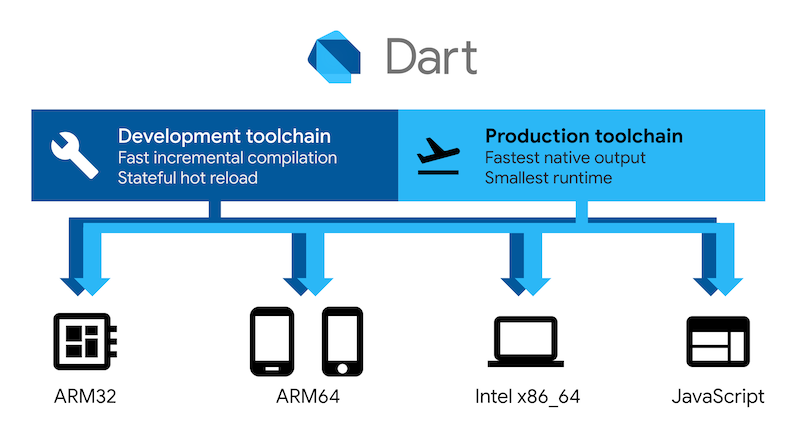
\includegraphics[scale=0.45]{Theoretische_Grundlagen/images/dart-diagram.png}
	\end{center}
	\caption{Kompatibilität der Dart Plattform \protect \footnotemark}
	\label{fig:dart_plattform}
\end{figure}
\footnotetext{Quelle: \url{https://github.com/flutter/flutter}}

\paragraph{Architektur}
\begin{displayquote}
	Flutter is designed as an extensible, layered system. It exists as a series of independent libraries that each depend on the underlying layer. No layer has privileged access to the layer below, and every part of the framework level is designed to be optional and replaceable.\footnote{\url{https://flutter.dev/docs/resources/architectural-overview}}
\end{displayquote}

Grundlegend ist das Framework in drei Prozesseinheiten gegliedert. Diese bestehen wiederum jeweils aus, für sie charakteristischen APIs und Bibliotheken:

\begin{itemize}
	\item \textit{Flutter embedder}: Der Einstiegspunkt in die jeweilige Plattform. Er koordiniert Zugriffe auf Services des Betriebssystems; er ist also zuständig für bspw. die Kommunikation mit dem Input Method Editor (IME) und den Lifecycle Events der App. Daher ist der Embedder in der, von der Plattform unterstützten Programmiersprache geschrieben: derzeit wird Java und C++ für Android, Objective-C/Objective-C++ für iOS und macOS, und C++ für Windows und Linux verwendet.
	\item \textit{Flutter Engine}: Der Kern von Flutter, geschrieben hauptsächlich in C und C++, ist die \textit{low-level} Implementierung der Flutter Kern Programmierschnittstelle (API). Daher ist sie zuständig für das graphische Darstellen (Rasterisierung) des Codes sobald ein neuer \textit{Frame} angezeigt werden muss. Im Flutter Framework wird die \textit{Engine} als dart:ui Bibliothek offengelegt - der zugrundeliegende C++ Code wird in Dart Klassen eingefügt. 
	\item \textit{Flutter Framework}: Das Framework, mit welchem der Entwickler schlussendlich meistens arbeiten wird. Es ist in Dart geschrieben und bietet sogenannte \textit{Layer} für Animationen, Layout und Widgets. Widgets werden von Flutter als Einheit der Komposition von Benutzeroberflächen verwendet und sind als einzelne Bausteine zu verstehen, welche zusammengefügt ein Objekt oder sogar einen kompletten Bildschirm ergeben.
\end{itemize}

Bei der Entwicklung mit Flutter wird ein Baum von Widgets erzeugt, welcher als Bauplan der Applikation angesehen werden kann. Nach diesem Plan wird mithilfe von States der einzelnen Widgets schlussendlich das User Interface (UI) gerendert.\cite{flutter2021}

\begin{figure}[tbt]
	\begin{center}
		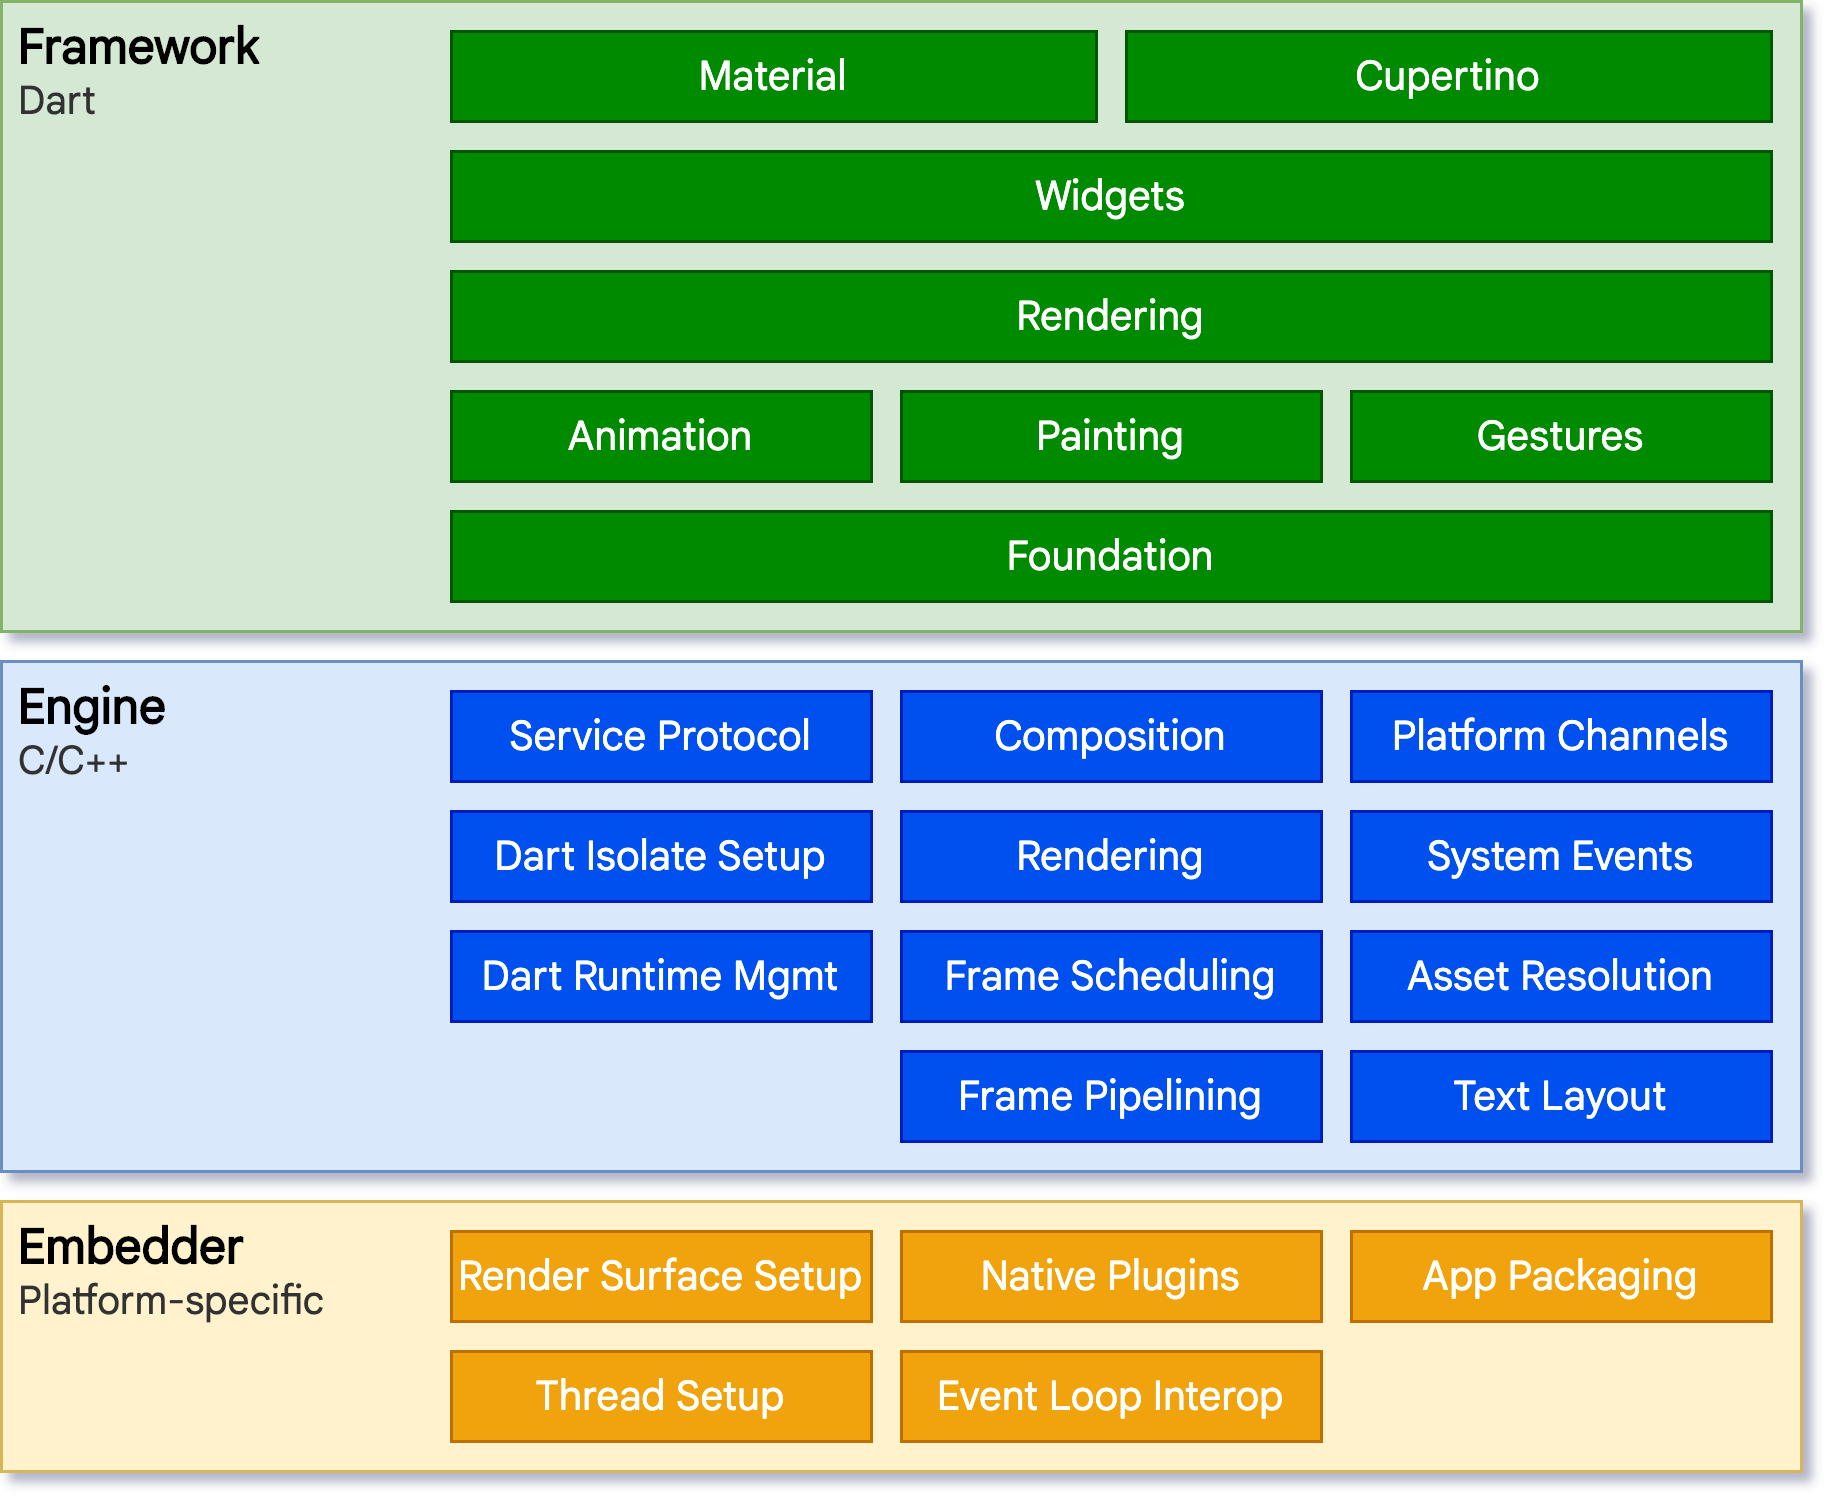
\includegraphics[scale=0.25]{Theoretische_Grundlagen/images/flutter_architektur.png}
	\end{center}
	\caption{Bibliotheken und Ebenen der Flutter Plattform \protect \footnotemark}
	\label{fig:flutter_plattform}
\end{figure}
\footnotetext{Quelle: \url{https://github.com/flutter/flutter}}

\paragraph{Dart}
Während der Entwicklung von Flutter standen sicherlich mehrere Sprachen zur Auswahl: \\Wie in Kapitel \ref{plattformuebergreifende_anwendungen} gelernt, gibt es viele unterschiedliche Ansätze mit beispielsweise webbasierten Sprachen wie JavaScript, mit nativen Sprachen wie Java oder Swift, oder auch mit anderen objektorientierten Sprachen wie C\#. Wieso wurde also genau Dart als Programmiersprache und Runtime ausgewählt?\\
\\
Dart allgemein ist C ähnlich, also für viele Entwickler leicht(er) leserlich. Es ist eine objekt-orientierte Sprache und besitzt einen Garbage Collector.\\
Dart ist designet als eine Client-fokussierte Sprache, welche gleichermaßen Entwicklung (sub-second stateful hot reload) und Produktion in allen möglichen Zielplattformen (Web, Mobile und Desktop) priorisiert. Dadurch erhält man mit dieser Sprache eine Effizienz optimierte Entwicklungsphase, sowie ebenfalls die Möglichkeit eine Code-Basis in unterschiedliche Plattformen zu kompilieren (siehe Abbildung \ref{fig:dart_plattform}).\\
Es bietet zudem auch \textit{sound-null-safety} - Werte können also nicht null sein, außer man legt dies fest. Damit kann es null Exceptions während der Laufzeit durch statische Code Analyse vorbeugen.

\paragraph{Widgets}
Wie bereits beschrieben sind Widgets wiederverwendbare Kompositionsbausteine, mit welchen Benutzeroberflächen in Flutter zusammengebaut werden. Jedes einzelne ist ein \textit{immutable declaration} eines Teils der Benutzeroberflächen - also ein konstanter Bestandteil.\\
\\
Flutter arbeitet mit der Devise: 
\begin{displayquote}
	\textbf{\textit{Everything is a widget.}}
\end{displayquote}
Auf diesem Satz baut die Einfachheit von Flutter auf. Jedes Objekt, jede Animation, jede Reihe, einfach alles ist ein Widget. Somit baut man eine App von der Wurzel aus auf und beschreibt die einzelnen Abzweigungen exakt.
Die Anordnung von Widgets ist daher hierarchisch aufgebaut. 
Ein Widget wir also immer in einem Elternteil verschachtelt sein und erhält bei seiner Erstellung den \textit{build context} übergeben. Das \glqq äußerste\grqq \space Widget, also die Wurzel, enthält somit die gesamte App. Typischerweise ist das ein \textit{MaterialApp} oder \textit{CupertinoApp} Widget.\\
\\ 
OEM Widgets, also Widgets von und für eine spezifische Plattform werden von Flutter gemieden. Hierfür erzeugt Flutter eigene Widgets mithilfe der oben genannten, eigener Rendering Plattform. Da diese Widgets jedoch komplett individualisierbar sind, bietet man somit native Möglichkeiten für jegliche Stile. Es gibt auch Pakete, welche Plattform-ähnliche Widgets zur Verfügung stellen.

\begin{figure}[tbt]
	\begin{center}
		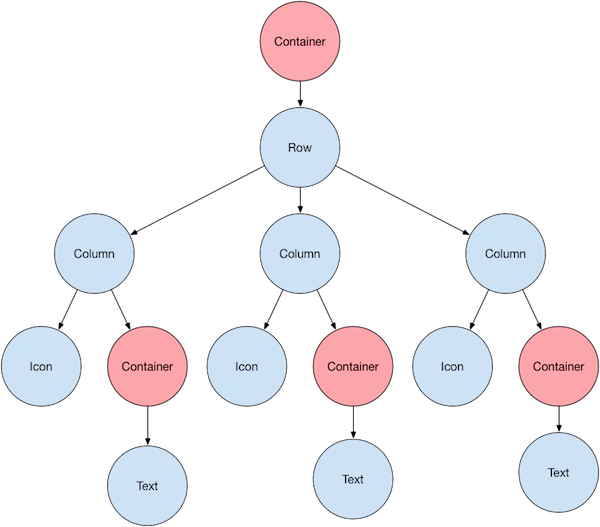
\includegraphics[scale=0.5]{Theoretische_Grundlagen/images/flutter_widget_tree.png}
	\end{center}
	\caption{Widget Baum einer beispielhaften Anwendung \protect \footnotemark}
	\label{fig:flutter_widget_tree}
\end{figure}
\footnotetext{Quelle: \url{https://flutter.dev/docs/development/ui/layout}}
	

\paragraph{States}
Flutter ist deklarativ - das bedeutet, die Benutzeroberfläche wird anhand von dem aktuellen \textit{State} der App erzeugt. Im Gegensatz dazu muss der Entwickler beim imperativen Stil die Übergänge der einzelnen \textit{States}. Hier wird dies durch das Framework gelöst.
	
\begin{figure}[H]
	\begin{center}
		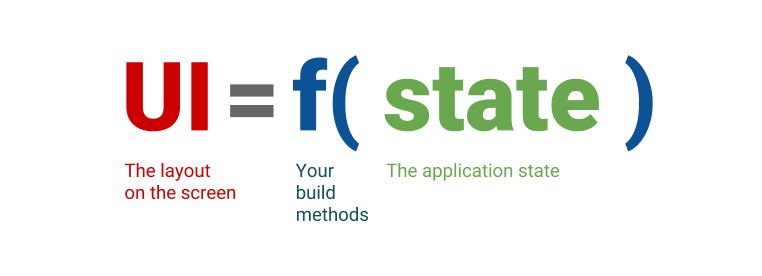
\includegraphics[scale=0.4]{Theoretische_Grundlagen/images/flutter_state.png}
	\end{center}
	\caption{Deklarative Benutzeroberfläche \protect \footnotemark}
	\label{fig:flutter_state}
\end{figure}
\footnotetext{Quelle: \url{https://flutter.dev/docs/development/data-and-backend/state-mgmt/declarative}}







